% !TeX encoding = UTF-8
\chapter{解的长时间演化行为}\label{chap4}

\section{概率解与稳定解}

类似于离散或连续Markov模型,随机过程长时间演化有可能收敛到一个均匀的概率分布,即极限状态与平稳状态存在且两者一致. 目前对如下形式的 SDE 已经有了一定的理论成果,
\begin{equation}\label{eq_sde_fokker}
	\md X_t = b(X_t) \md t + \sigma(X_t) \md B_t,\qquad  x\in \R^d. 
\end{equation}
注意到它是自治随机偏微分方程,也就是说,其解的转移过程可以用一个Markov转移半群来表述\cite{semi_group_1,semi_group_2},而与时间项 $t$ 无关. 
借助 Feynman-Kac 表示,它可以与 Fokker-Planck 型确定型微分方程建立起紧密的联系. 令 $(a^{ij}) := \frac12 \sigma\sigma^T$. Fokker-Planck 方程的形式为:
\begin{equation}\label{eq_fokker}
	\partial_t u = Lu := \sum_{i,j=1}^d \partial^2_{ij} (a^{ij}u) - \sum_{i=1}^d \partial_i (b^ix),\qquad
	t>0,x \in \R^d.
\end{equation}

我们利用(\ref{eq_fokker})来定义(\ref{eq_sde_fokker})的测度意义下的弱解和稳定解.首先定义 Fokker-Planck 算子的伴随算子
\begin{equation}\label{eq4.3}
	\mL = \sum_{i,j}a^{ij} \partial_{ij}^2  + \sum_i b^i \partial_i
\end{equation}

\begin{definition}[测度解]
	令 $\nu$ 是 $\R^n$ 上的Borel测度. 我们称一族Borel测度 $\mu = (\mu_t)_{t\in [0,T]}$ 是问题(\ref{eq_sde_fokker})的初值为 $\nu$ 的测度解,若 $\mu_0=v$,$a^{ij},b^i \in L^1_{\mathrm{loc}}(\R^n,\md \mu_t \md t) \quad \forall i,j $ 且下面恒等式在$[0,T]$上几乎处处成立
	\[
	\int_{\R^n} \phi \md \mu_{t}=\int_{\R^n} \phi \md \nu + \lim _{\varepsilon \to 0^{+}} \int_{\varepsilon}^t \int_{\R^n} \mL \phi \md \mu_s \md s,\quad \phi \in C_{0}^{\infty}(\R^n) .
	\]	
	进一步地,若 $\mu_t(\R^n) = 1$,则称为概率解. 
\end{definition}

此处的概率解 $\mu=(\mu_t)$ 代表问题(\ref{eq_sde_fokker})在初值 $X_0$ 服从概率分布 $\mu_0$ 时解 $(X_t)$ 的概率分布. 因而测度具有归一化的性质. Feynman-Kac 表示的成立对漂移项和扩散项函数有一定的要求,此处不再多做介绍. 
Fokker-Planck 方程的概率解的存在性和唯一性已经在很多文献中进行了讨论\cite{zongshu2-24,zongshu2-26},包括系数函数与时间 $t$ 相关的问题. 
接下来定义样本轨道的集合的稳定状态. 这里在概率意义下给出稳定解的定义:






\begin{definition}[稳定解]
	$\R^n$ 上的 Borel 测度 $\mu$ 称为稳定解,若 Fokker-Planck 方程(\ref{eq_fokker})对应的算子 $L$ 满足 $L\mu = 0$,即
	$b_i \in L^1_{\text{loc}}(\R^n , \mu), \forall i$ 且
	\[
	\int_{\R^n} \mL \phi \md \mu = 0,\qquad  \forall \phi \in C_0^\infty(\R^n).
	\]
\end{definition}

不同于之前从样本轨道的角度理解方程的解,概率解和稳定解从所有样本轨道的角度出发理解随机微分方程解的性质. 







\begin{definition}[Lyapunov 型函数]
	对 $\R^d$ 上的非负连续函数 $U \in C^2(\R^d)$,记水平集
	\[
	\Omega_\rho = \{ x\in \R^d :U(x) < \rho \},\qquad \rho > 0,
	\]
	其为准紧集. 
	\begin{enumerate}
		\item 称无界函数 $U$ 为 Lyapunov 型函数,若存在常数 $C_1,C_2,\rho_m > 0$ 使得
		\[
		\mathcal{L} U(x) \leq C_{1}+C_{2} U(x), \quad x \in \R \backslash \overline {\Omega}_{\rho_{m}}
		\]
		\item 称无界函数 $U$ 为 Lyapunov 函数,若存在常数 $\gamma,\rho_m>0$ 使得
		\[
		\mathcal{L} U(x) \leq-\gamma, \quad x \in \R \backslash \overline {\Omega}_{\rho_{m}}
		\] 
		\item 称无界函数 $U$ 为强 Lyapunov 型函数,若存在常数 $C_1,C_2,\rho_m > 0$ 使得
		\[
		\mathcal{L} U(x) \leq C_{1}-C_{2} U(x), \quad x \in \R \backslash \overline {\Omega}_{\rho_{m}}
		\]
	\end{enumerate}
\end{definition}

这三种条件逐步加强,概率解的存在性和唯一性的定理如下:

\begin{theorem}
	若存在算子 $\mL$ 对应的 Lyapunov 型函数,则下列叙述成立:
	\begin{enumerate}
		\item
			方程(\ref{eq_fokker})存在初值概率分布为 $\nu$ 下的概率解 $(\mu_t)_{t\in[0,\infty)}$,且对任意 $\phi \in C_0^\infty(\R^d)$,映射 $t\mapsto \displaystyle \int_{\R} \phi \md \mu_t$ 是连续的;  
		\item 
			若 $(\tilde \mu_t)_{t\in [0,\infty)}$ 也是方程(\ref{eq_fokker})在初值概率分布为 $\nu$ 下的概率解,且满足映射 $t\mapsto \displaystyle \int_{\R} \phi \md \tilde\mu_t$ 是连续的对任意 $\phi \in C_0^\infty(\R^d)$ 成立,则 $\tilde \mu_t = \mu_t,\quad  \forall t>0$. 
	\end{enumerate}
\end{theorem}



上述定理说明了方程(\ref{eq_fokker})的概率解的存在唯一性,Feynman-Kac 公式表明随机的SDE的解与Fokker-Planck方程的解能关联起来. 因此SDE到达稳定状态时,$\partial_t\mu(t,x) = 0$. 注意到
\[
\int_{\R^n} \mL \phi \md \mu = \int_{\R^n} (\mL \phi, \mu(t,x)) \md x= 
\int _{\R^n} (\phi,L\mu(t,x)) \md x = 0.
\]
因此在弱意义下,有 $\partial_t \mu = L\mu = 0$. 















\section{稳定解验证}
%文献指出\cite{Fokker_Planck}指出,稳定解存在和收敛的充分条件是存在区域范围上无界非负 Lyapunov函数 $U(x)$ 和常数 $C_1,C_2>0 $,使得
%\[
%\mL U(x) \le C_1 - C_2 U(x) \qquad \text{或} \qquad 
%\mL U(x) < -C_1.
%\]


文献\cite{Fokker_Planck}指出,在 Lyapunov 条件下,自治随机微分方程(\ref{SODE})存在稳定解,且概率解在强 Lyapunov 条件下以指数速率收敛到稳定解. 
\begin{theorem}
	下面叙述成立:
	\begin{enumerate}
		\item
			若存在算子 $\mL$ 对应的无界 Lyapunov 函数,当 $t\to\infty$ 时,方程(\ref{eq_fokker})的任意测度解 $(\mu_t)_{t\in[0,\infty)}$ 均强收敛到唯一的稳定解 $\mu^*$,即对任意 Borel 可测集 $B \in \R^d$,有
			 \[
			 \mu_t(B) \to \mu^*(B),\qquad t\to \infty.
			 \]
		\item
			若存在算子 $\mL$ 对应的无界强 Lyapunov 函数,当 $t\to\infty$ 时,无论初值测度 $\nu$ 如何,测度解 $(\mu_t)_{t\in[0,\infty)}$  均指数收敛到唯一的稳定解 $\mu^*$,即存在常数 $C,r > 0$,使得
			\[
			\left\|\mu_{t}-\mu^{*}\right\|_{\operatorname{TV}} \leq C e^{-r t}, \quad t \geq 0,
			\]
			这里 $\|\cdot\|_{\operatorname{TV}} $ 表示全变差范数. 
	\end{enumerate}
\end{theorem}



简单看两个稳定解存在的例子和一个稳定解不存在的例子.

\subsection*{例1}
考虑方程
\[
\md x = bx \md t + \sqrt{2\sigma(x^2+1)} \md B_t,
\]
其中 $\sigma > b > 0$. 则其对应的 Fokker-Planck 方程为
\[
\partial_t = Lu := \partial_{xx} (\sigma(x^2+1)u) - \partial_x (bxu).
\]
取 $U(x) = \ln(x^2+1)$,伴随算子 $\mL = \sigma(x^2+1)\partial_{xx} + bx\partial_x$,有
\[
\mL U(x) = -\frac{2(\sigma-b) x^{2}-2 \sigma}{x^{2}+1} \le -(\sigma-b).
\]
满足 Lyapunov 条件,因此稳定解存在. 取参数$(b,\sigma)=(2,5)$,有偏初值 $X_0=10$,即 $P(X_0 = 10) = 1$,对 $50000$ 条样本轨道进行模拟,采用Milstein格式,结果见图\ref{path_4_1}和\ref{measure_4_1}.
一直模拟到 $T=100$,解始终维持 $T=5$ 时的形态. 再看另一个稳定解的例子. 

若不考虑噪声项,则 $x_t = x_0 e^{bx}$,随机系统退化为一个指数爆炸的系统,但引入充分大($\sigma>b$)的噪声项后,数值实验表明尽管样本轨道的二阶矩是发散的,但 $t$ 时刻绝大部分的点会落于 $[-10,10]$ 内. 

\begin{figure}[!htbp]
	\centering 
	\subfigure[T=0.001]{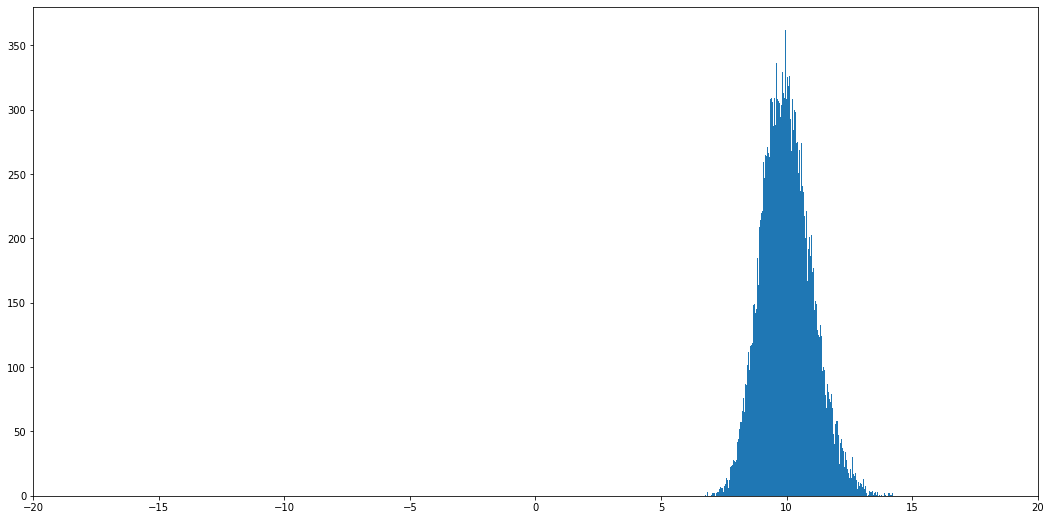
\includegraphics[width=2.95in]{images/4.1/fig_4.1(T=0.001)}}
	\subfigure[T=0.005]{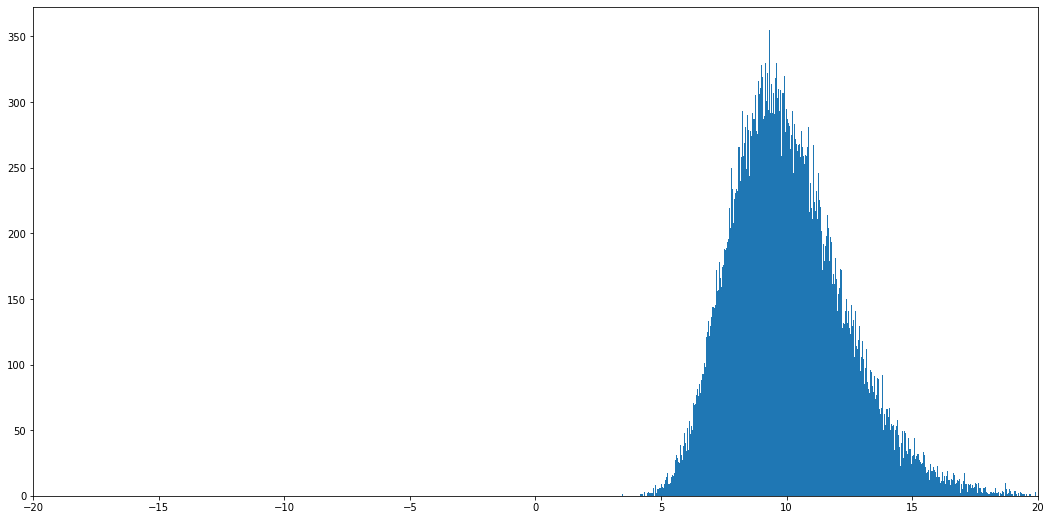
\includegraphics[width=2.95in]{images/4.1/fig_4.1(T=0.005)}}
	\subfigure[T=0.01]{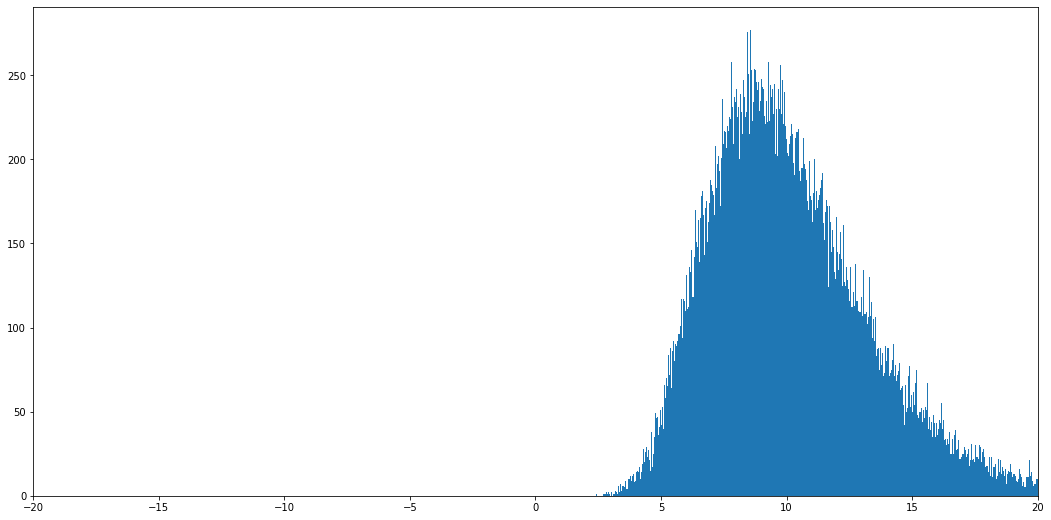
\includegraphics[width=2.95in]{images/4.1/fig_4.1(T=0.01)}}
	\subfigure[T=0.05]{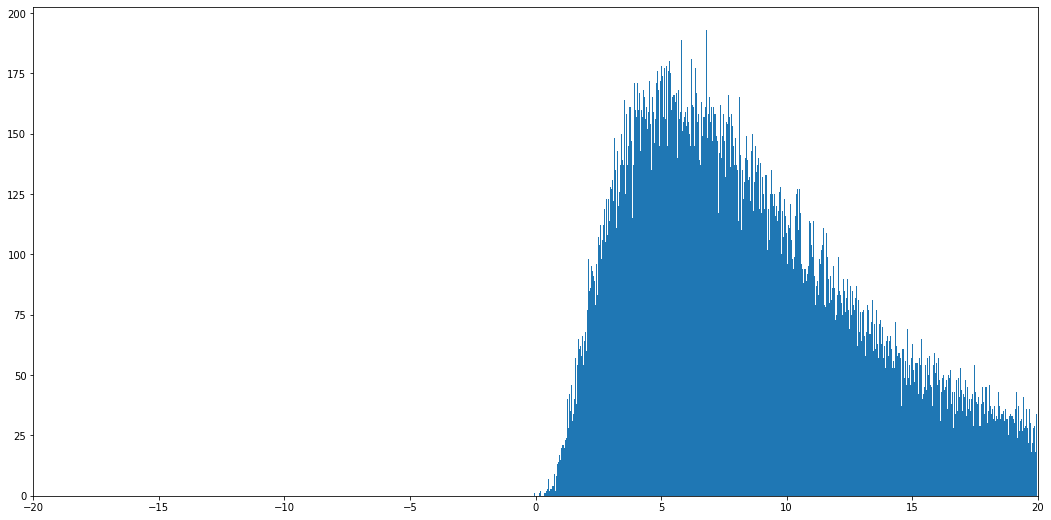
\includegraphics[width=2.95in]{images/4.1/fig_4.1(T=0.05)}}
	\subfigure[T=0.1]{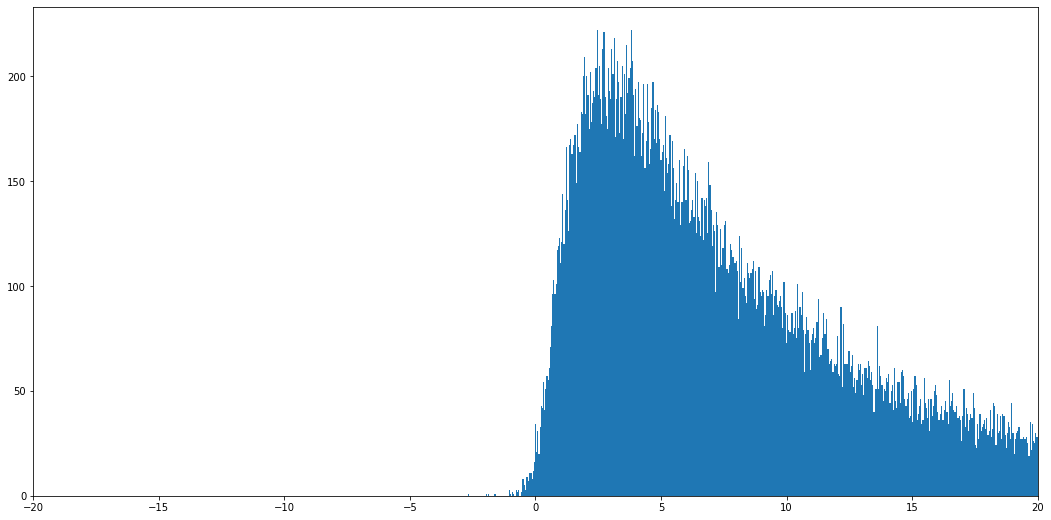
\includegraphics[width=2.95in]{images/4.1/fig_4.1(T=0.1)}}
	\subfigure[T=0.5]{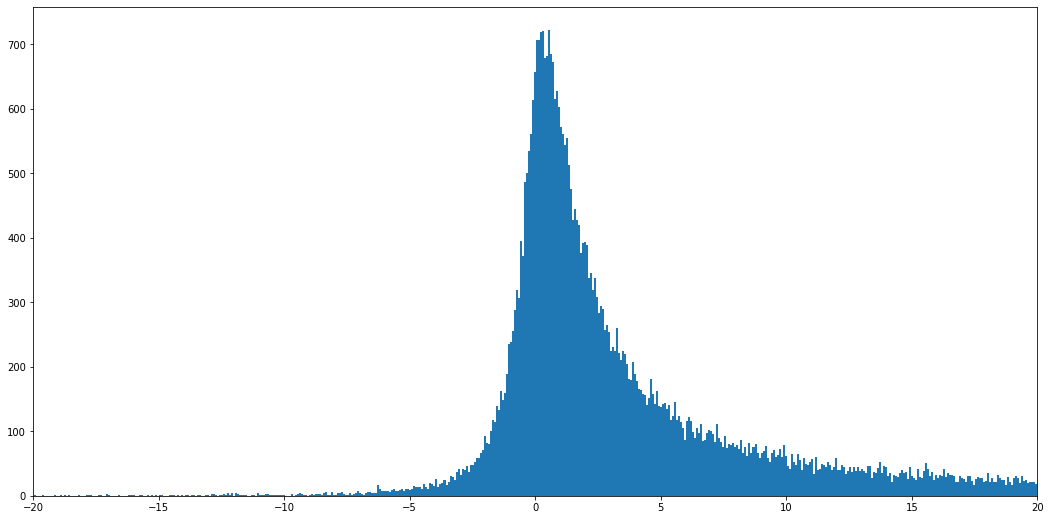
\includegraphics[width=2.95in]{images/4.1/fig_4.1(T=0.5)}}
	\subfigure[T=1]{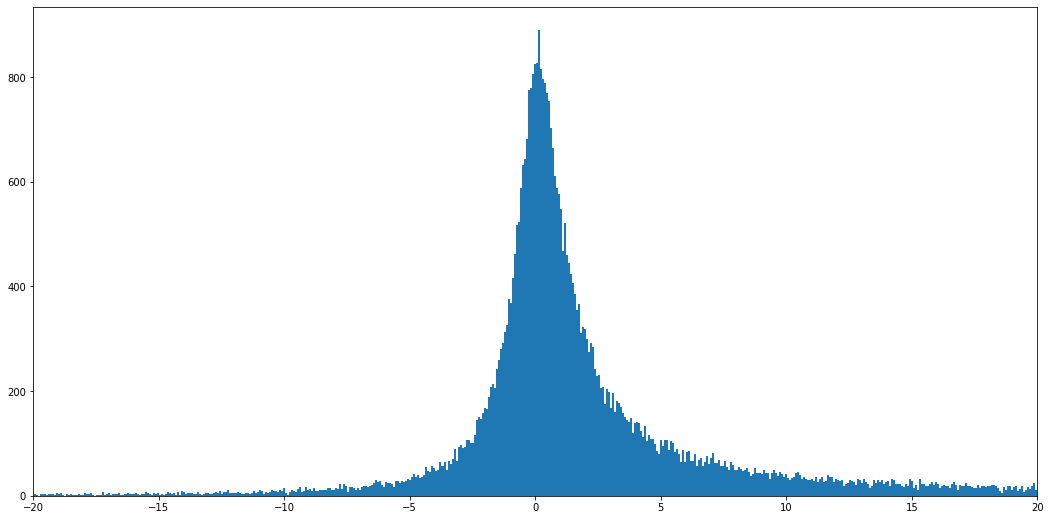
\includegraphics[width=2.95in]{images/4.1/fig_4.1(T=1)}}
	\subfigure[T=5]{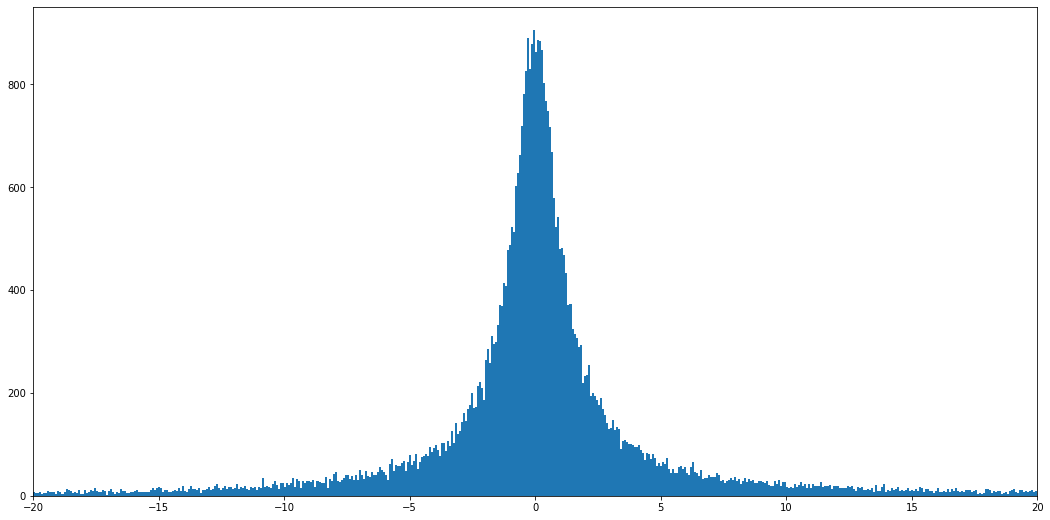
\includegraphics[width=2.95in]{images/4.1/fig_4.1(T=5)}}
	\centering
	\vspace{.2cm}
	\caption{稳定解的概率分布(一)}
	\label{measure_4_1}
\end{figure}

\begin{figure}[!htbp]
	\centering 
	\subfigure[样本轨迹1]{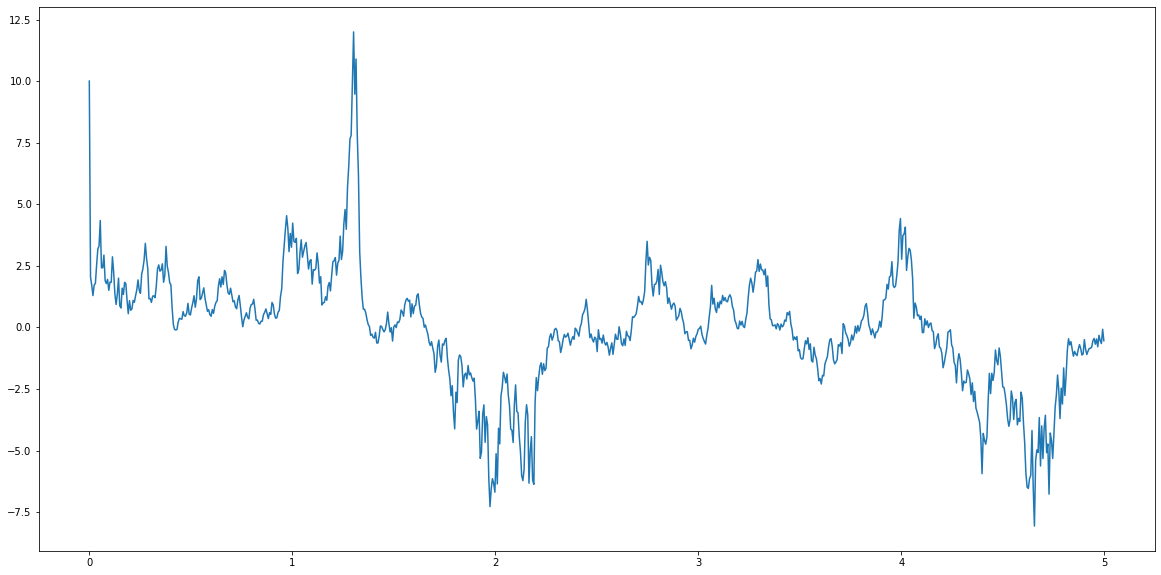
\includegraphics[width=2.95in]{images/4.1/path_4.1.1}}
	\subfigure[样本轨迹2]{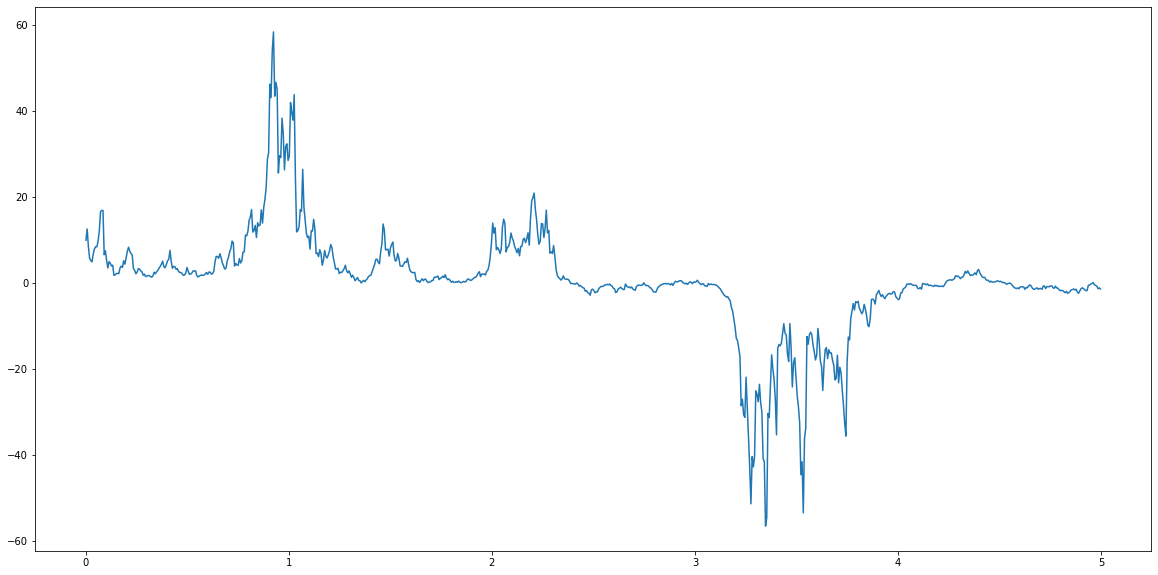
\includegraphics[width=2.95in]{images/4.1/path_4.1.2}}
	\vspace{.2cm}
	\caption{存在稳定解的样本轨道}
	\label{path_4_1}
\end{figure}





\subsection*{例2}
考虑方程
\[
 \md x = bx \md t + \sqrt{2} (1-x^2)\md B_t ,\qquad x\in(-1,1)
\]
其中 $b<0$. 
该随机系统的值域落在$(-1,1)$内.这是因为当 $x \to 1^-$ 或 $x\to (-1)^{+}$ 时,扩散项会收缩到0,而漂移项给予该随机系统一个向着0回归的趋势,同时,任意的样本轨道都是连续的,使得系统无法“跳跃”过 $-1$ 和 $1$ 两个点. 
选取 Lyapunov 函数为 $U(x) =  -\ln(1-x^2)$,
\[
\mL U(x) = 2+2x^2+\frac{2bx^2}{1-x^2},
\]
当 $|x| \to 1^-$ 时,$\mL U(x) \le 3 + 2b U(x)$,从而满足强 Lyapunov 条件. 

\begin{figure}[!htbp]
	\centering 
	\subfigure[T=0.00]{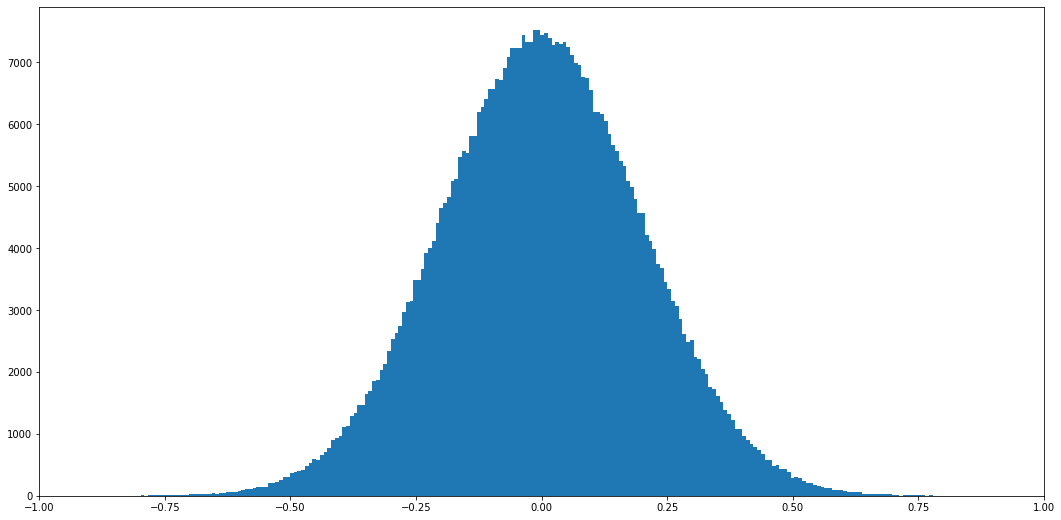
\includegraphics[width=1.45in]{images/4.2/fig_4.2(T=0.00)}}
	\subfigure[T=0.01]{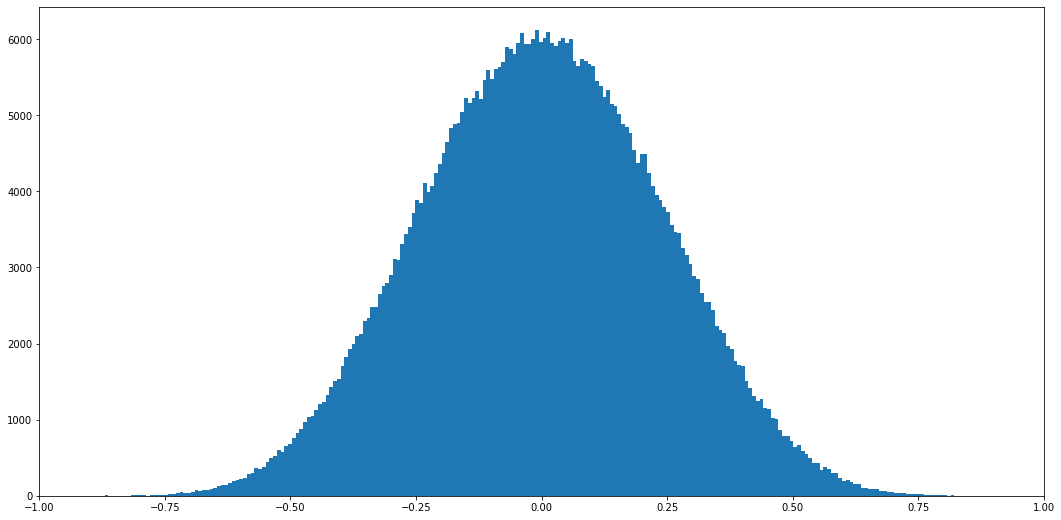
\includegraphics[width=1.45in]{images/4.2/fig_4.2(T=0.01)}}
	\subfigure[T=0.02]{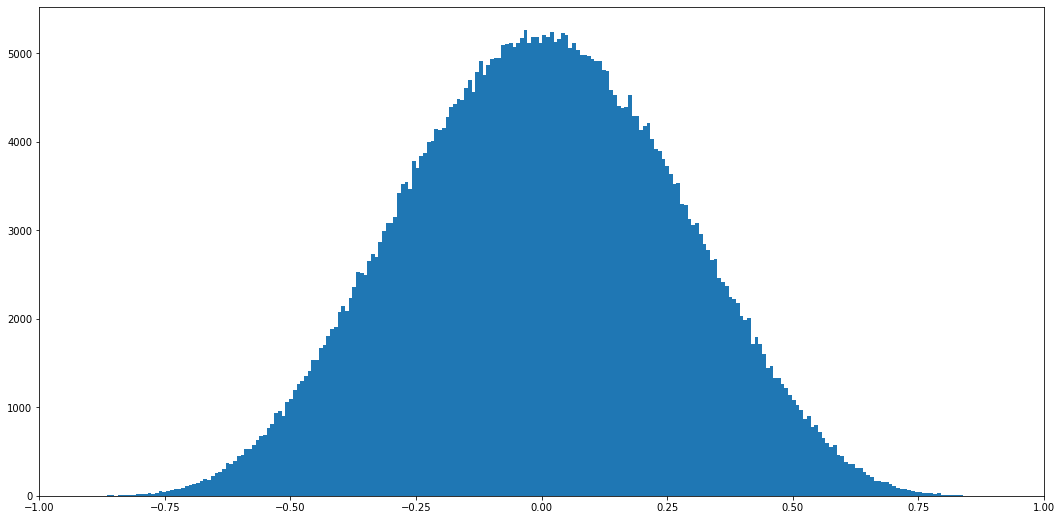
\includegraphics[width=1.45in]{images/4.2/fig_4.2(T=0.02)}}
	\subfigure[T=0.05]{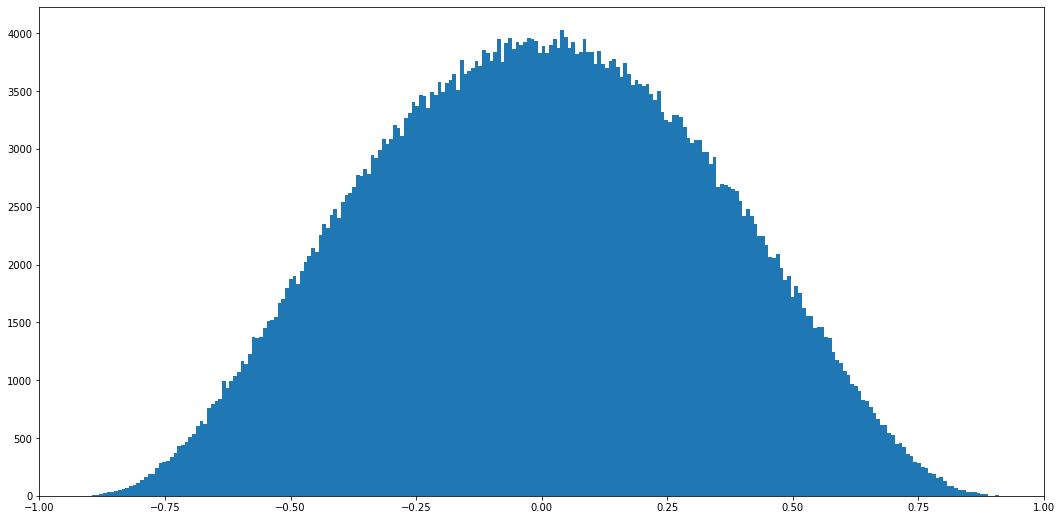
\includegraphics[width=1.45in]{images/4.2/fig_4.2(T=0.05)}}
	\subfigure[T=0.10]{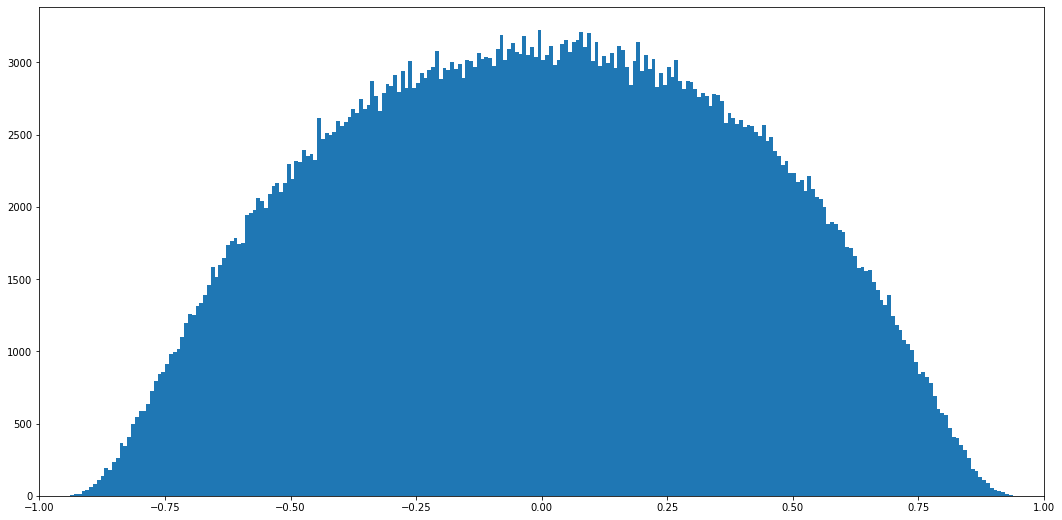
\includegraphics[width=1.45in]{images/4.2/fig_4.2(T=0.10)}}
	\subfigure[T=0.20]{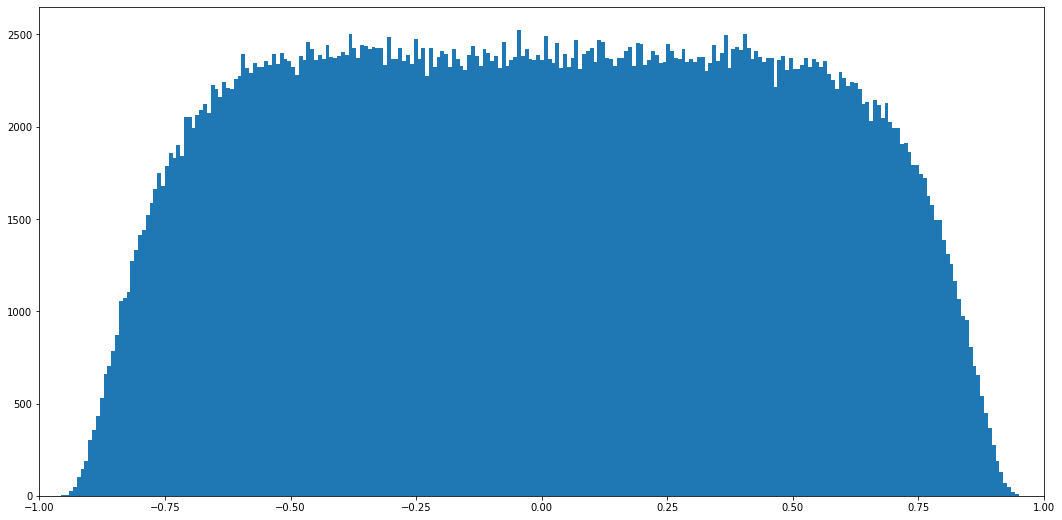
\includegraphics[width=1.45in]{images/4.2/fig_4.2(T=0.20)}}
	\subfigure[T=0.50]{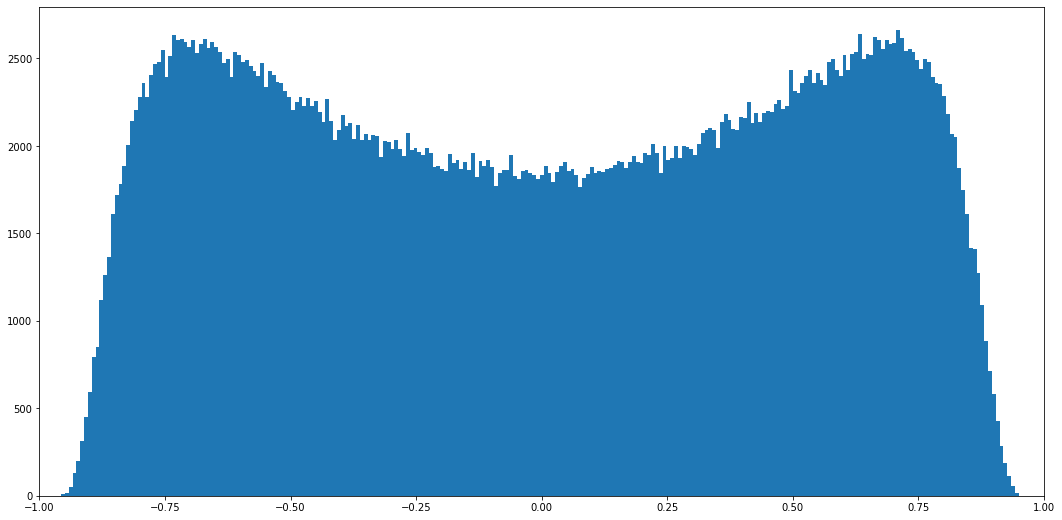
\includegraphics[width=1.45in]{images/4.2/fig_4.2(T=0.50)}}
	\subfigure[T=1.00]{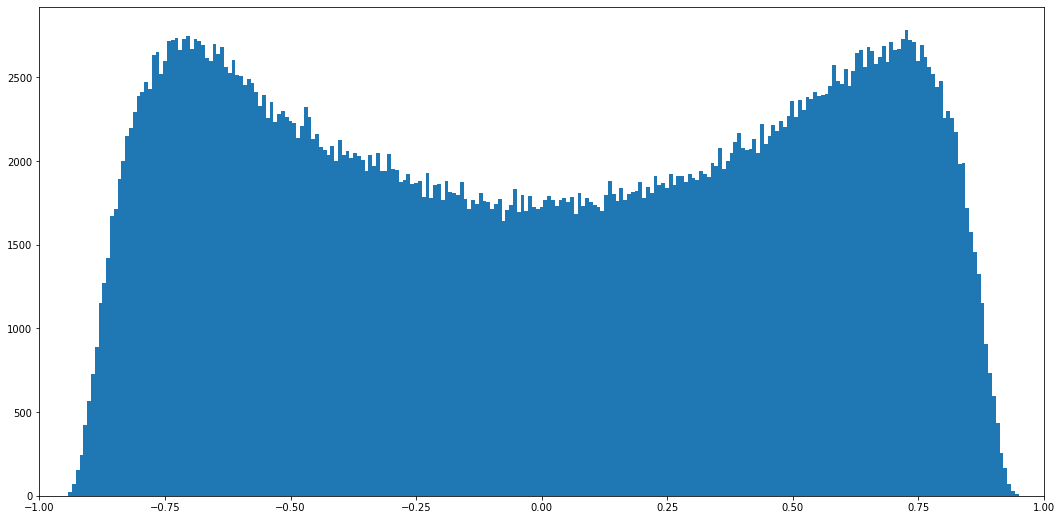
\includegraphics[width=1.45in]{images/4.2/fig_4.2(T=1.00)}}
	\subfigure[T=2.00]{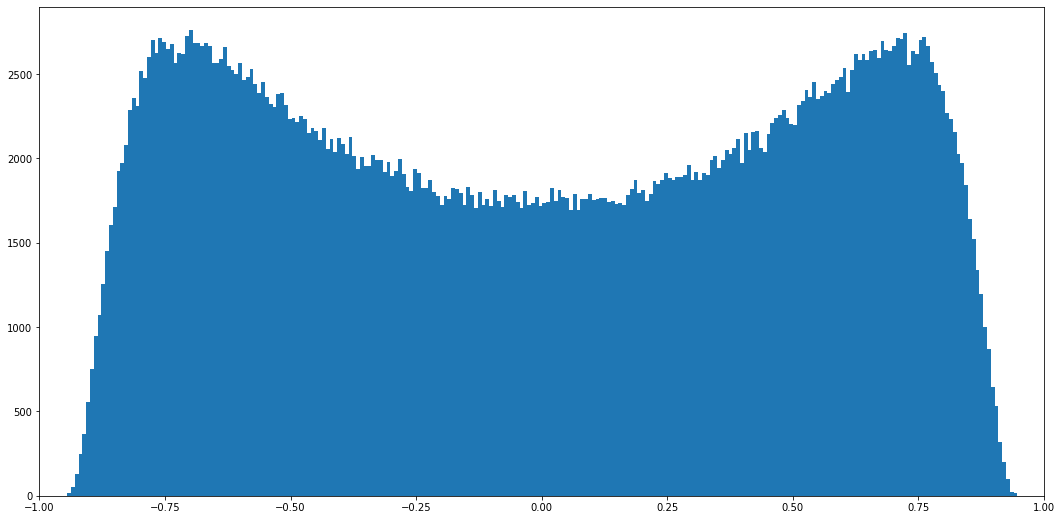
\includegraphics[width=1.45in]{images/4.2/fig_4.2(T=2.00)}}
	%\subfigure[T=4.00]{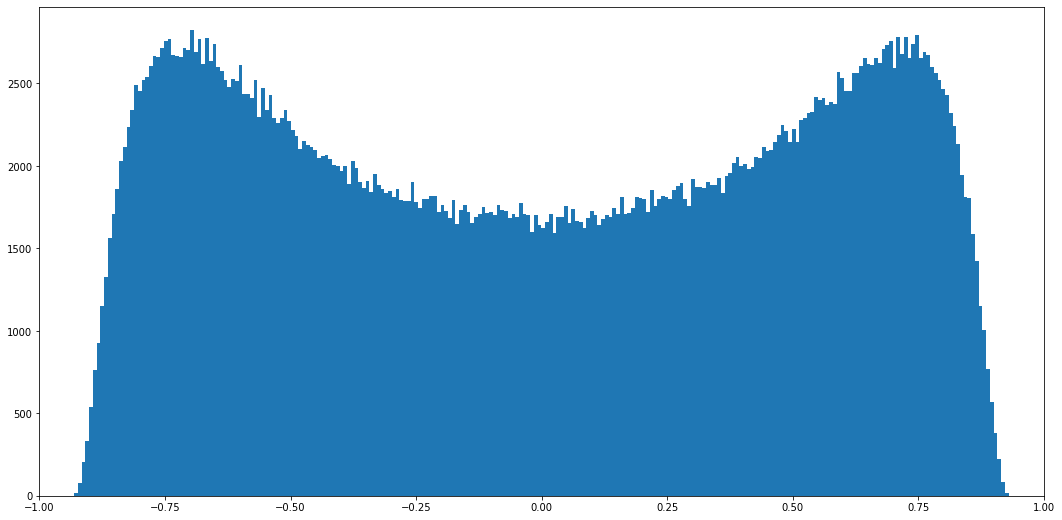
\includegraphics[width=1.45in]{images/4.2/fig_4.2(T=4.00)}}
	\subfigure[T=5.00]{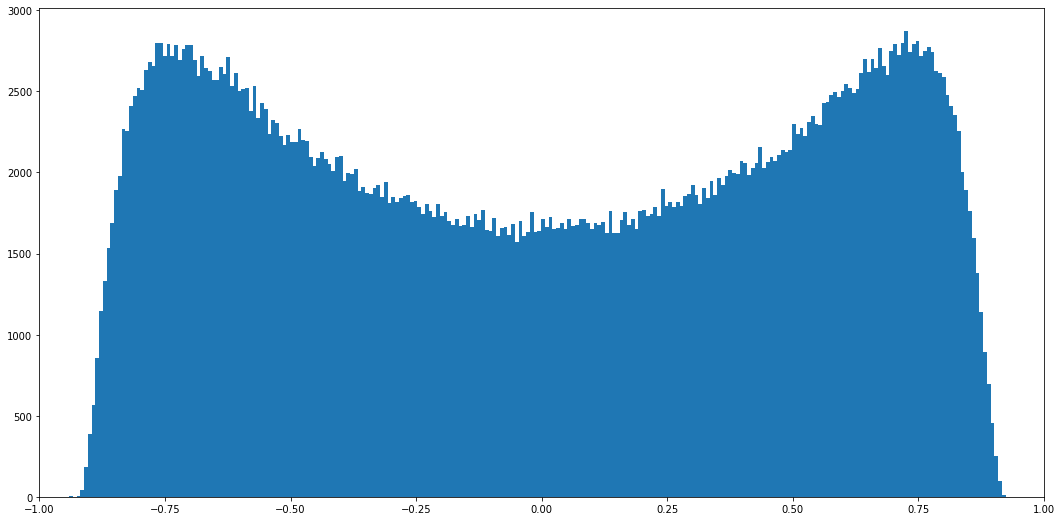
\includegraphics[width=1.45in]{images/4.2/fig_4.2(T=5.00)}}
	%\subfigure[T=8.00]{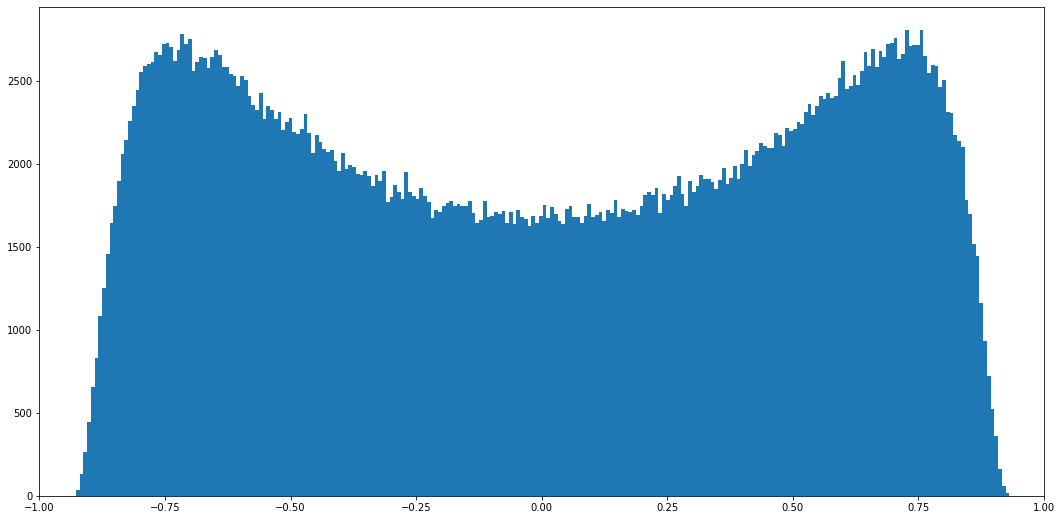
\includegraphics[width=1.45in]{images/4.2/fig_4.2(T=8.00)}}
	\subfigure[T=10.0]{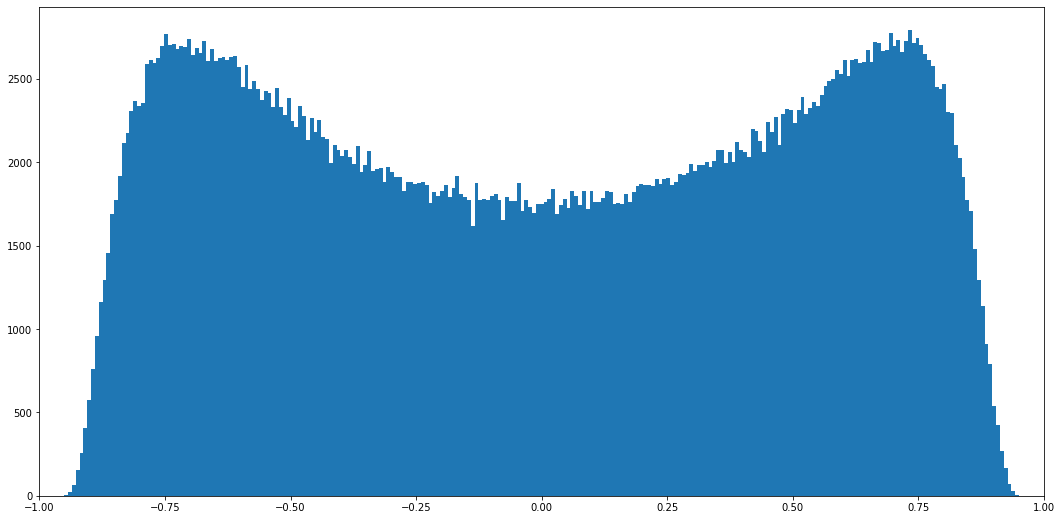
\includegraphics[width=1.45in]{images/4.2/fig_4.2(T=10.0)}}
	\subfigure[T=20.0]{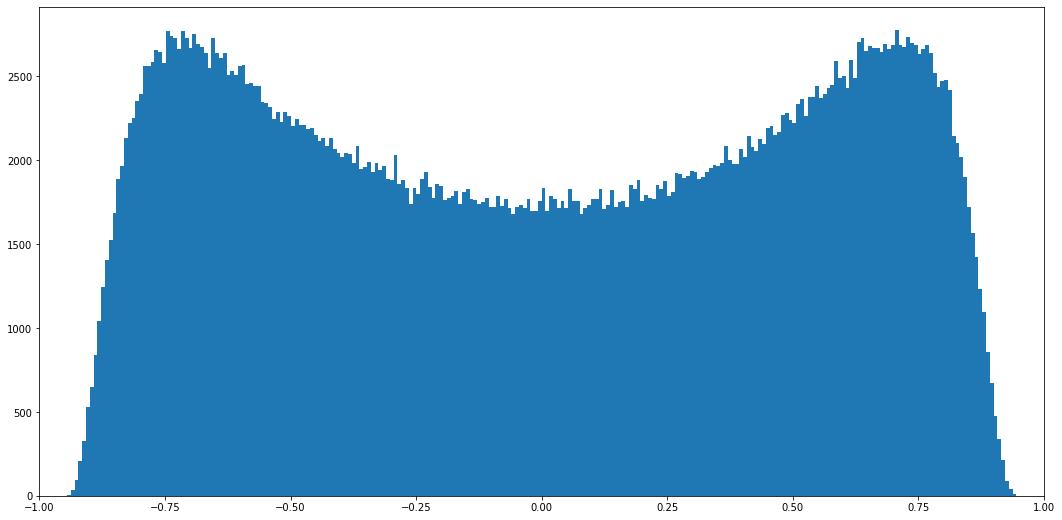
\includegraphics[width=1.45in]{images/4.2/fig_4.2(T=20.0)}}
	\centering
	\vspace{.2cm}
	\caption{稳定解的概率分布(二)}
	\label{measure_4_2}
\end{figure}

数值实验选取初值 $X_0$ 为正态分布 $N(0,0.2)$,并除去落在 $(-1,1)$ 以外的不合理的样本点,模拟结果见图\ref{measure_4_2},可以看出随机系统长时间演化后形成了特定的概率分布. 


\subsection*{例3}
并非所有 SDE 都存在稳定解,如下面的随机微分方程的概率解就会不断扩散,
\[
\md X = \sin(X) \md t + \sqrt{2} \md B_t,\qquad P(X_0 = 0)=1.
\]
\begin{figure}[!htbp]
	\centering 
	\subfigure[T=1]{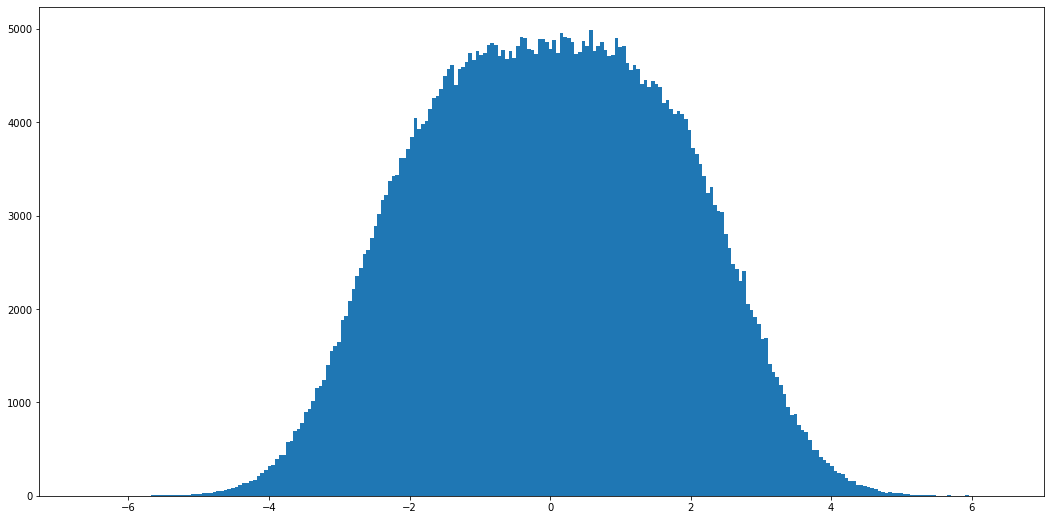
\includegraphics[width=1.45in]{images/4.3/fig_4.3(T=1)}}
	\subfigure[T=5]{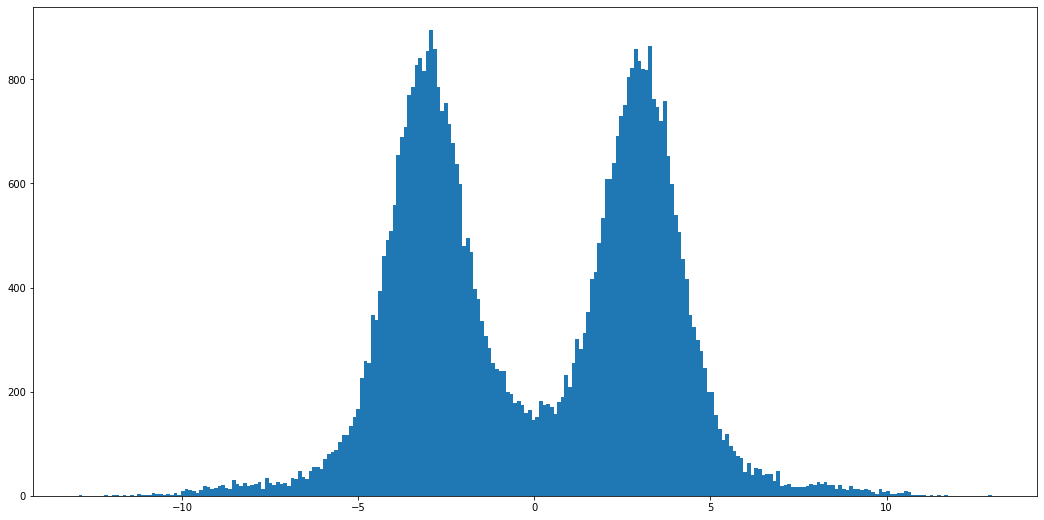
\includegraphics[width=1.45in]{images/4.3/fig_4.3(T=5)}}
	\subfigure[T=10]{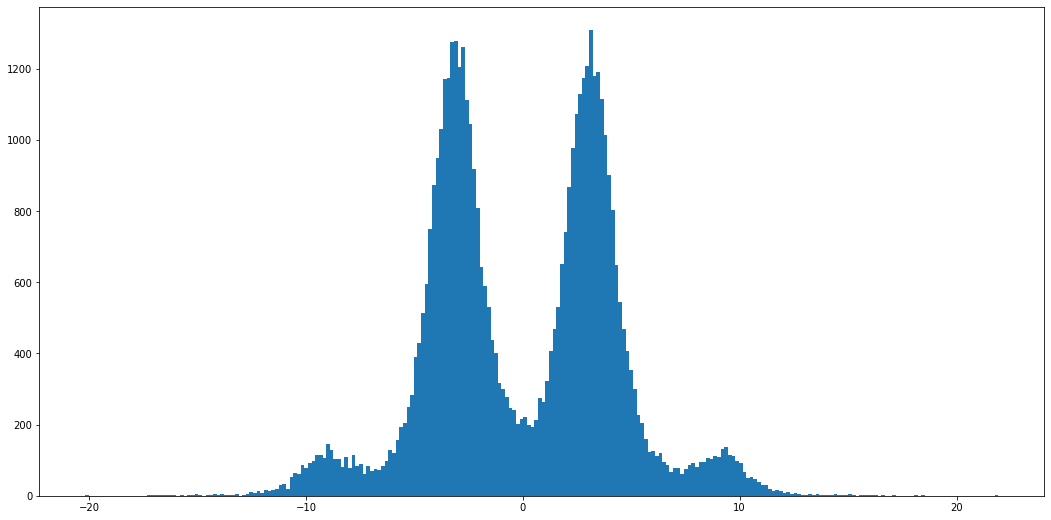
\includegraphics[width=1.45in]{images/4.3/fig_4.3(T=10)}}
	\subfigure[T=50]{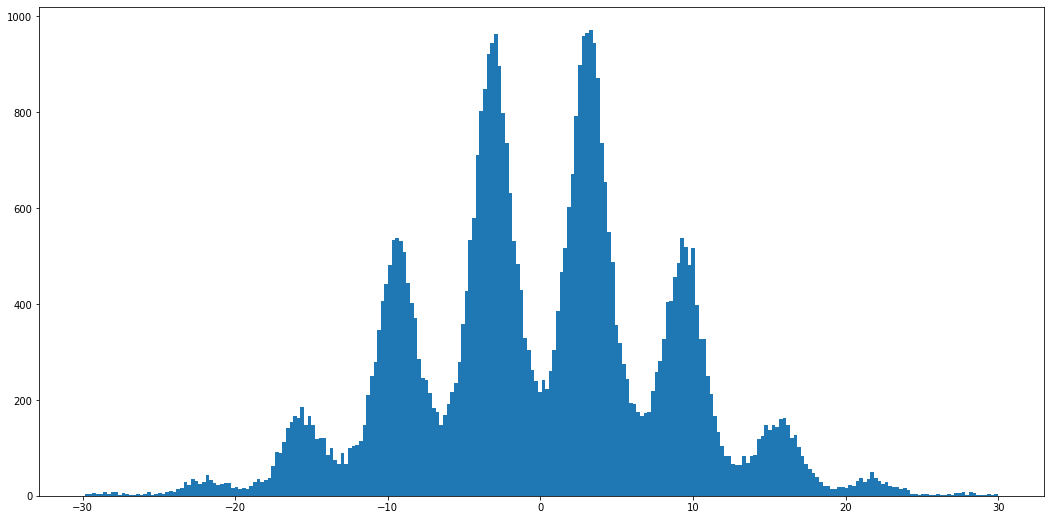
\includegraphics[width=1.45in]{images/4.3/fig_4.3(T=50)}}
	\centering
	\vspace{.2cm}
	\caption{不存在稳定解的概率分布}
	\label{measure_4_3}
\end{figure}
与之前两个可以生成稳定解的例子不同,该例中随机系统的漂移项和扩散项不会互相制约,使得系统达到一个稳定的状态. 
稳定解对应转移方程 $T_{t_0} \mu = \mu$,即稳定解在自治系统作用时间 $t_0$ 后概率分布维持不变,而该系统不存在这样的概率分布. 


\section{稳定解的加速算法}
对于自治随机微分方程,若存在稳定解,考虑初始概率分布 $\mu_0$ 和经过时间 $t$ 之后得到的概率分布为 $\mu_t$,两者具有同样的稳定概率分布 $\mu^*$.也就是说,两个不同的初始概率分布具有一致的稳定解. 
当稳定解唯一时,即算子 $\mL$ 对应的方程的解唯一时,自治随机微分方程在任意初值条件下均能达到稳定解. 现考虑稳定解唯一的情况,本节探讨稳定解的数值算法. 

随机微分方程数值解的模拟很费时间,对于收敛速度慢的随机系统,全程使用较小的步长 $h$ 会使得总计算时长大大增加;而全程使用较大的步长 $h$,则会导致误差较大. 文献\cite{Fokker_Planck}指出,若满足强 Lyapunov 条件,稳定解的收敛速度是甚至指数级的,即:
\[
	\| \mu_t -\mu^* \|_{\operatorname{TV}} \le Ce^{-rt}. 
\]
而 $p$ 阶单步算法导出的概率解 $\tilde \mu_t$ 是失真的. 但只要满足
\[
	\| \tilde{ \mu} _t - \mu_t \|  + \| \mu_t -\mu^* \|  < \| \mu_0 -\mu^* \| ,
\]
则该过程的演化仍然是有价值的. 这是因为失真的的概率解 $\tilde\mu_t$ 并不会影响最终的稳定解. 
注意到 $\| \tilde \mu_t - \mu_t \| $ 的精度是 $O(h^p)$,而计算时间是 $O(\frac1h)$. 因此设计如下数值算法:

\begin{algorithm}[!htbp]
	\caption{稳定解的加速算法}%算法名字
	\LinesNumbered %要求显示行号
	\KwIn{SDE 系统,误差界$\varepsilon$,样本轨道数$N$}%输入参数
	%\KwOut{output result}%输出
	$X = \mathcal N(0,1,N),\quad h=0.1,\quad \rm{time} = 0$\;
	\For{\rm{i in \{0,1,2,…,10\}}}{
		h = h / 2 \;
		M = pow(2,i)\;
		\For{\rm{j in \{0,1,2,…,M\}}}{
			time = time + h\;
			newX = scheme(X,h)\;
			\If{$\|\rm{sort(newX)-sort(X)}\| < \varepsilon$}{
				break\;
			}\Else{
				newX = X\;
			}
		}
	}
\end{algorithm}

当稳定解唯一时,稳定解的初值无关性带来极大的好处,算法运行初期引入的误差是不会影响最终的解,但使用较大的步长 $h$ 可以使程序快速收敛到稳定解附近,而后续过程将 $h$ 取的较小,又可以使得精度相较普通方法更高. 


但如果稳定解不唯一,数值实验表明该算法不一定会收敛. 本文下一章节针对一类稳定解存在但不唯一的随机系统,提出了相应的求解稳定解的加速算法. 














